%*******************************************************************************AA
%*********************************** Chapter XXXXXXXX *****************************
%*******************************************************************************

\nomenclature[z-PoCA]{PoCA}{Point of Closest Approach} 

\chapter{Simulations of the DUNE Far Detector}  %Title of chapter
\graphicspath{{FarDetectorSimulations/Figs/Raster/}{FarDetectorSimulations/Figs/PDF/}{FarDetectorSimulations/Figs/}}

Previous work presented has been done concerning the 35 ton prototype, however it is also important to simulate the DUNE Far Detector (FD). Simulations in the FD have concentrated on cosmogenic background to neutrino oscillations, in Section~\ref{sec:LBNESurf}, and the muon background to nucleon decay, in Section~\ref{sec:DUNENDK}. The simulations shown in Section~\ref{sec:LBNESurf} are discussed in!!!!~citep{MartinsThesis}!!!!, and were performed for the Long Baseline Neutrino Experiment (LBNE), which along with the Long Baseline Neutrino Oscillation (LBNO) experiment, formed the basis for DUNE, and so are included here for completeness. The other work presented was performed for the DUNE collaboration, in conjunction with work done by Vitaly Kudryavtsev and Matthew Robinson, both of the University of Sheffield. This work was performed with the aim of producing muon-induced background limits to nucleon decay in the DUNE FD. \\

%********************************** %Second Section  **************************************
\section{Simulations of the LBNE surface detector} \label{sec:LBNESurf} %Section - X.2

%********************************** % Third Section  *************************************
\section{The use of MUSUN in LArSoft} \label{sec:FDIncorporation}  %Section - X.3
The primary muons in the following discussions are all generated using MUSIC~\citep{MUSUN}~\citep{MUSIC}~\citep{MUSIC2} and MUSUN~\citep{MUSUN}~\citep{MUSUN2}, and so a brief overview of them is required. MUSIC first propagates muons through a medium, defined by the user, for given initial energies, positions, and direction cosines. A range of energies between 10$^2$ and 10$^7$ GeV are considered, and their energy distributions are stored at depths of between 100 and 15,000 m w.e. Energy losses due to four processes are considered; ionisation, bremsstrahlung, electron-positron pair production and muon-nucleus inelastic scattering. The output of MUSIC is then used by MUSUN to generate a muon energy spectrum and angular distribution, for a given detector location. MUSUN is able to use information about the local surface profile to make these distributions more accurate. \\

The location of the DUNE far detector, near the Ross shaft at SURF, has global coordinates of, 44$^{\circ|}$20$'$45.21$''$ North, 103$^{\circ}$45$'$16.13$''$ West. The rock composition is assumed to be, $< Z >$ = 12.09 and $< A >$ = 24.17. The density is assumed to be 2.70 g cm${-3}$~\citep{Mei:2009py}. The flux calculated by MUSIC/MUSUN of 5.18 $\times$ 10$^{-9}$ cm$^{-2}$ s$^{-1}$ sr$^{-1}$, is well matched to the flux measured by the active veto system of the Davis' experiment, which was (5.38 $\pm$ 0.07) $\times$ 10$^{-9}$ cm$^{-2}$ s$^{-1}$ sr$^{-1}$~\citep{PhysRevD.27.1444}. Given the small differences in these values, and another measurement by the Majorana demonstrator, the systematic uncertainty in calculating the muon flux is estimated to be 20\%~\citep{NDKTFNote}. \\

The surface profile around the proposed detector location is shown in Figure~\ref{fig:SurfProf_Col}, where the proposed location is in the centre of the map. Each quadrant on the map has been divided into 4 angles of 22$^{\circ}$, to help guide the eye when comparing it to Figure~\ref{fig:SurfProf_Azi}, where the distribution of azimuth angles is plotted. The vertical lines in Figure~\ref{fig:SurfProf_Azi} show the division of the quadrants when the angle is calculated from East to the North. When moving from East to North it is possible to discern how the peaks and troughs on the surface profile, correspond to troughs and peaks, in the distribution of azimuthal angle. \\

\begin{figure}[h!]
  \centering
  \begin{subfigure}{0.45\textwidth}
    \centering
    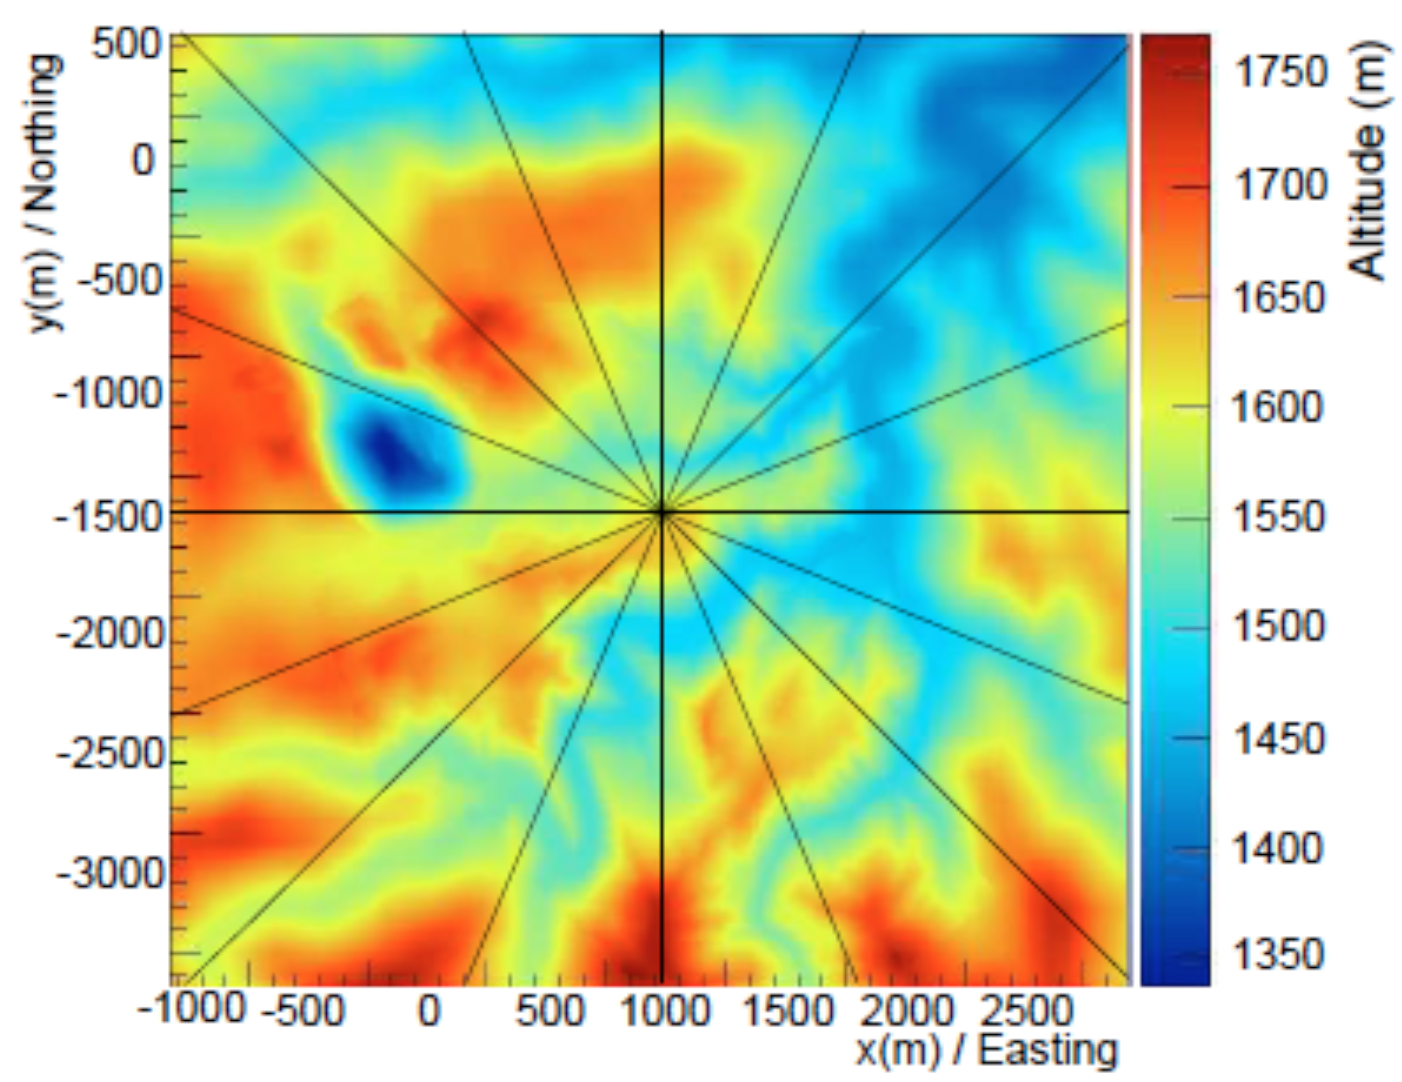
\includegraphics[width=\textwidth]{dune-surface-map}
    \caption{The surface profile of the DUNE far detector site at SURF.}
    \label{fig:SurfProf_Col}
  \end{subfigure}
  \hspace{0.08\textwidth}
  \begin{subfigure}{0.45\textwidth}
    \centering
    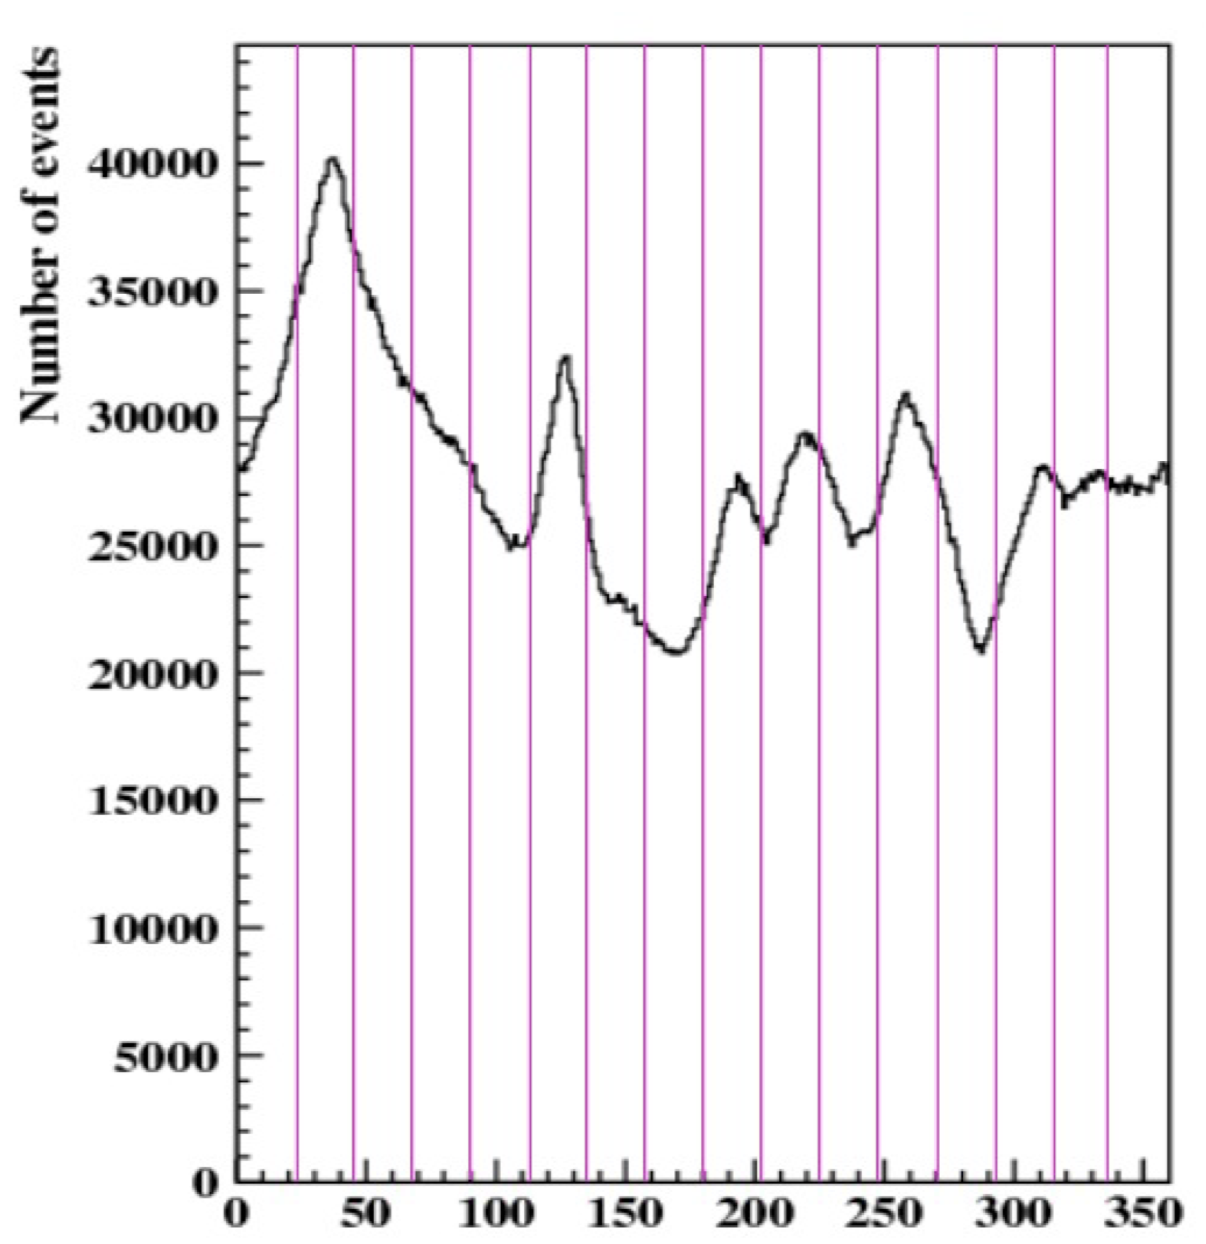
\includegraphics[width=\textwidth]{phi-map}
    \caption{The distribution of azimuthal angles of muons at the DUNE far detector site at SURF.}
    \label{fig:SurfProf_Azi}
  \end{subfigure}
  \caption[The correlation between the surface profile and distribution of azimuthal angles at the DUNE far detector site]
          {The correlation between the surface profile and distribution of azimuthal angles at the DUNE far detector site. The quadrants have been divided into four angles of equal size. The azimuthal angle, calculated as the angle from East (pointing to the right in Fig.~\ref{fig:SurfProf_Col}), and increasing counterclockwise, is seen to follow the contours of the surface profile.}
\end{figure}

Given these parameters, the muon flux at the DUNE far detector location, when assuming a spherical detector geometry, and without simulating a detector cavern, is given by Table~\ref{tab:MUSUNflux}. \\
\begin{table}[h!]
  \caption[Muon flux parameters as calculated with MUSIC/MUSUN.]
          {Muon flux parameters as calculated with MUSIC/MUSUN.}
  \centering
  \label{tab:MUSUNflux}
  \begin{tabular}{c c c c}
    \toprule
        {Total flux (cm$^{-2}$ s$^{-1}$)} & {Mean E$_{\mu}$ (GeV)} & {Mean slant depth (m w.e)} & {Mean $\theta$ ($^{\circ}$)} \\ 
        \midrule
        5.66 $\times$ 10$^{-9}$           & 283                    & 4532                       & 26                           \\
    \bottomrule
  \end{tabular}
\end{table}

The muons simulated for DUNE are sampled on the surface of a box surrounding the detector hall, that also encompasses 7 m of rock above the cavern, and 5 m of rock on all other sides. This is to ensure that the simulated muons pass through a sufficient amount of rock to induce cascades, both above and around the detector hall. The secondaries produced in these cascades which enter the detector, in the absence of the initial muon, are of particular interest, as they could be mistaken for nucelon decay events. The study of these nucelon decay mimicking events is discussed in Section~\ref{sec:DUNENDK}. The size of the box which the muons are sampled from is 74.43 $\times$ 29.54 $\times$ 30.18 m$^3$, compared to the simulated cryostat which has dimensions, 61.62 $\times$ 14.94 $\times$ 13.58 m$^3$. The dimensions are given as length $\times$ width $\times$ height. The muons are sampled randomly according to their energy spectrum, for a given zenith and azimuthal angle, using the angular distribution obtained with MUSIC. \\

Before this could be done however, MUSUN had to be incorporated into the DUNE software framework, as it had previously been maintained in FORTRAN as an external package. This involved building on the work done by the LZ collaboration in porting the code to C++~!!!!!citep{Kareem}. The process by which this was done, was to first reproduce the distributions produced by the LZ collaboration using the DUNE software framework. Once the distributions could be reproduced for the Davis shaft at SURF, the muon distributions produced by the original FORTRAN code for the DUNE detector location were reproduced. The distributions produced by the DUNE software framework are shown in Figure~\ref{fig:MUSUNIncorp}. These are seen to be consistent with the distributions made for the LBNE collaboration~\citep{MUSUNLBNE}. The initial positions of 10,000 muons generated in LArSoft around the simulated DUNE 10 kt module are shown in Figure~\ref{fig:10ktPos}. The initial positions of the muons are shown as blue points, whilst the cryostat is a single black box, and each TPC is a single red box. \\

\begin{figure}[h!]
  \centering
  \begin{subfigure}{0.45\textwidth}
    \centering
    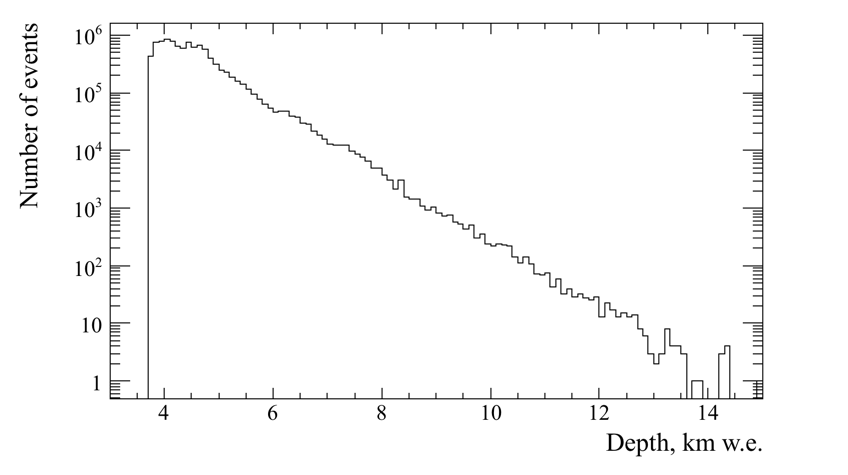
\includegraphics[width=\textwidth]{DepthCan}
    \caption{The number of muons with given slant depths.}
  \end{subfigure}
  \hspace{0.08\textwidth}
  \begin{subfigure}{0.45\textwidth}
    \centering
    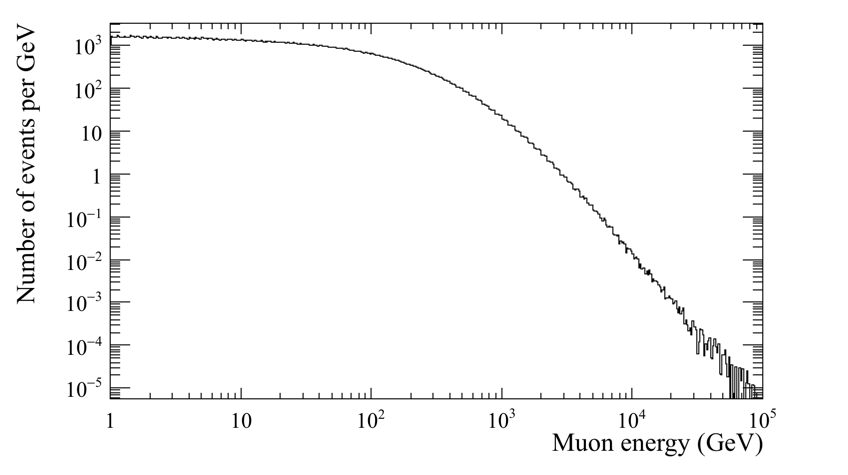
\includegraphics[width=\textwidth]{EnergyPerGeVCan}
    \caption{The initial energy spectrum of simulated muons.}
  \end{subfigure}
  % ========
  \begin{subfigure}{0.45\textwidth}
    \centering
    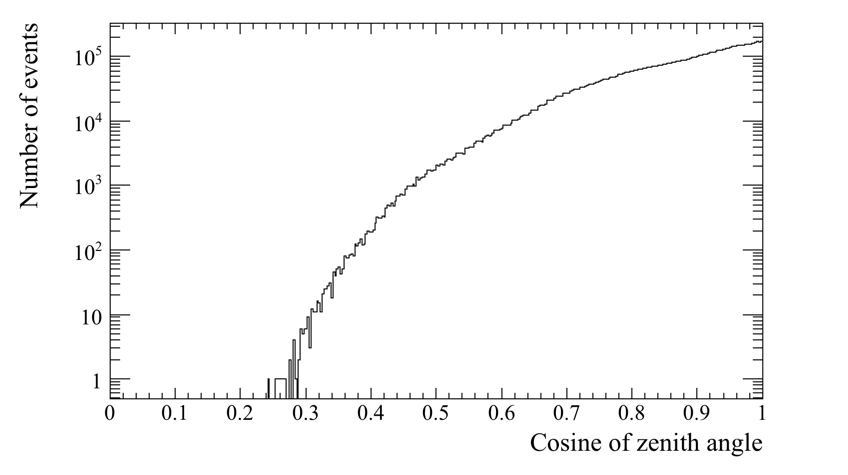
\includegraphics[width=\textwidth]{ZenithCan}
    \caption{The number of muons with given zenith angles.}
  \end{subfigure}
  \hspace{0.08\textwidth}
  \begin{subfigure}{0.45\textwidth}
    \centering
    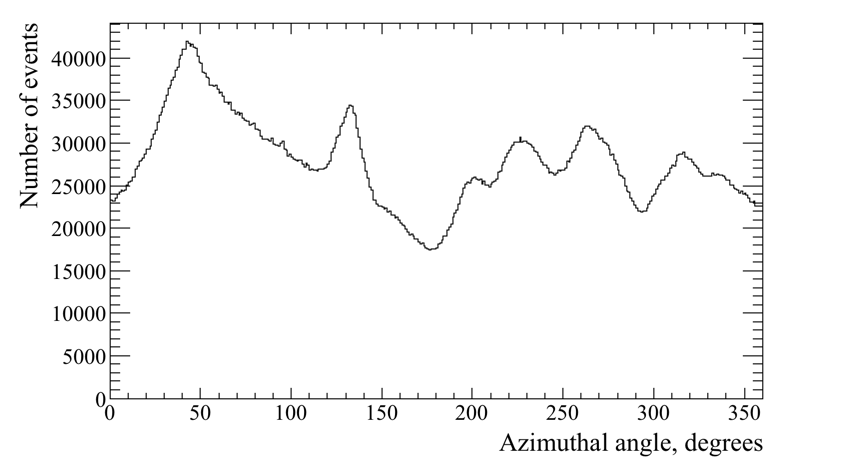
\includegraphics[width=\textwidth]{AzimuthCan}
    \caption{The number of muons with given azimuthal angles.}
  \end{subfigure}
  % ========
  \begin{subfigure}{0.45\textwidth}
    \centering
    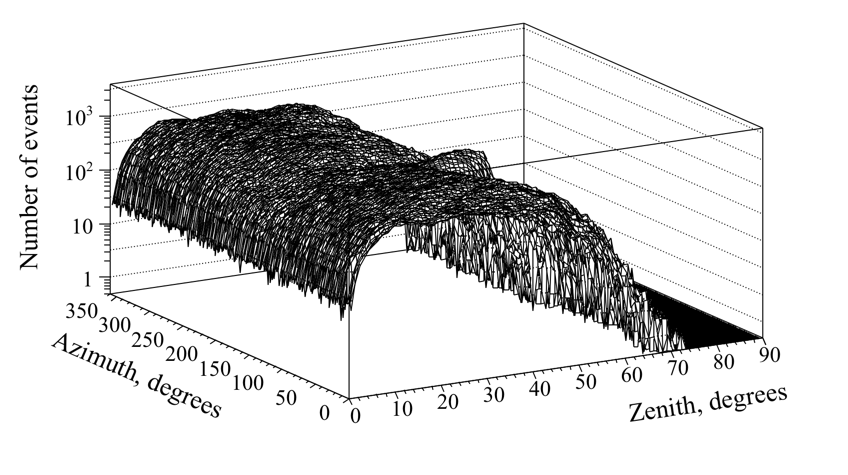
\includegraphics[width=\textwidth]{AziZenCan}
    \caption{The distribution of zenith and azimuthal angles.}
  \end{subfigure}
  \hspace{0.08\textwidth}
  \begin{subfigure}{0.45\textwidth}
    \centering
    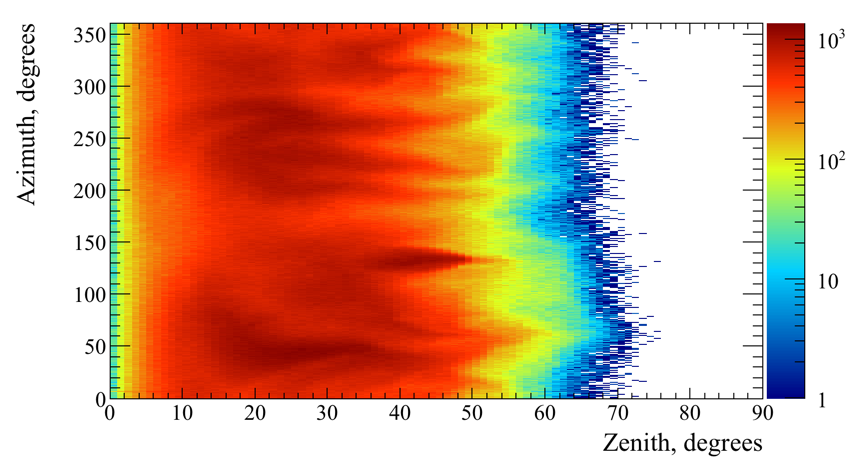
\includegraphics[width=\textwidth]{AziZenColzCan}
    \caption{The distribution of zenith and azimuthal angles, shown with a colour $z$ scale.}
  \end{subfigure}
  \caption[The distributions of some of the important quantities for a sample of 10$^6$ muons generated by MUSUN in LArSoft]
          {The distributions of some of the important quantities for a sample of 10$^6$ muons generated by MUSUN in LArSoft. The slant depths and energies of the simulated muons are shown top. The azimuthal and zentih angles of muons are shown middle. Bottom left shows the profile of zenith angle, against azimuthal angle, whilst bottom right shows this with a colour $z$ axis.}
  \label{fig:MUSUNIncorp}
\end{figure}

\begin{figure}[h!]
  \centering
  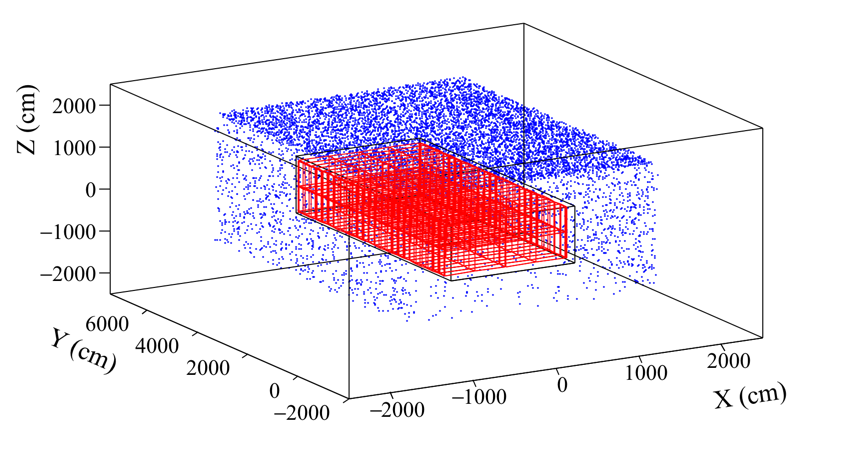
\includegraphics[width=\textwidth]{MuonPosCan}
  \caption[The initial positions of muons generated by MUSUN around a DUNE 10 kt module]
          {The initial positions of muons generated by MUSUN around a DUNE 10 kt module. The initial positions of the muons are shown as blue points, whilst the cryostat is a single black box and each TPC is a single red box.}
  \label{fig:10ktPos}
\end{figure}

It is found that the muon rate through the box upon which the muons are sampled is 0.1579 Hz. This rate is later used to normalise the background event rate in Section~\ref{sec:DUNENDK}. Roughly a third of the muons which are generated pass through the active volume, to give a muon rate through the active volume of 0.053 Hz. \\ 

%********************************** % Fifth Section  *************************************
\section{Nucleon decay channels in DUNE} \label{sec:DUNENDK} %Section - X.5
When searching for rare processes, where an experiment is unlikely to see more than a few real signatures, an exhaustive study of the potential backgrounds is required. This is so that if a signal is observed, it could provide overwhelming evidence for the process. The search for nucleon decay in DUNE is one such process, and so an exhaustive study of the background to nucleon decay is required. As discussed in Section~\ref{sec:BkNDK}, cosmogenic muons cause backgrounds to nucleon decay signatures, as the secondary particles produced by their interactions are able to mimic the nucleon decay signatures. For this reason it is necessary to simulate this background, and to develop a series of cuts which can be applied to the energy depositions they produce, to establish that they are not due to nucleon decays. When doing this, it is important to use a simulation that is as accurate as possible to the DUNE far detector. It is for this reason that MUSUN was incorporated into LArSoft, as the muons which it generates are well matched to the observed muon flux, as described in Section~\ref{sec:FDIncorporation}. \\

To ensure that the background has been properly simulated it is advantageous to simulate many more background events than will be collected by the experiment. As the DUNE detector will run for roughly 20 years, it was decided that an initial sample representing 200 years of detector live time would be simulated. Given that the muon rate through the cavern is 0.1579 Hz, 200 years of detector live time corresponds to roughly 10$^9$ muons. This only represents one of the DUNE 10 kt modules, and so an even larger dataset will be required to represent the full live time of the 4 10 kt modules. For this reason, muons were generated beyond this initial sample size, with a total of 2$/times$10$^9$ muons having been simulated currently. \\

Producing samples of this size requires significant computer power, both in terms of running time, and storage space. As such, many of the simulated events are discarded before being saved to disk, through the application of a filter after GEANT4. It is essential that the events which are discarded could not have been mistaken for nucleon decay events, and so only very generous cuts are applied. Only events satisfying one of the following cuts are discarded;
\begin{itemize}
\item Contain a muon track of more than 1 m.
\item There are no energy depositions in the entire detector volume.
\end{itemize}
It is envisioned that a muon track of more than a metre would not be misreconstructed. It is also assumed that any signatures observed within one drift window of such a track would not be studied in a nucleon decay search, as there would be doubt as to the authenticity of the signal. Given that the total rate of muons through the active volume is 0.053 Hz, and that the drift time is a few ms, ignoring all times where any track from a cosmogenic muon is present results in less than 0.1\% dead time. The dead time associated with ignoring events with muon tracks of more than 1 m is clearly less than this. This amount of dead time is assumed to be acceptable. \\

After applying this series of cuts, the sample of 2$/times$10$^9$ muons is reduced to XXXX$\times$10$^{XXXX}$ muons, which is a much more reasonable sample size to store on tape, and to perform analyses on. It is upon this reduced sample of muons that the cosmogenic background analyses are performed. As discussed in Section~\ref{sec:NDK_Atmos}, the proton decay channel of $p \rightarrow K^{+} + \nu^{e}$ is referred to as the 'Golden Channel' in LAr, this analysis is discussed in~\citep{NDKTFNote}. The related decay of channel of $n \rightarrow K^{+} + e^{-}$ is discussed here. \\

%********************************** % Fifth.First Section  *************************************
\subsection{Cosmogenic background to the $n \rightarrow K^{+} + e^{-}$ decay channel} \label{sec:NDKCosmBk}
As shown in Table~\ref{tab:NDKLim}, the predicted sensitivity that DUNE will have to this channel is much larger than that of Super-K. As a result, it is an interesting decay mode to study as DUNE could easily have the best limit for this decay channel. As discussed in Section~\ref{sec:BkNDK}, the cosmogenic background to nucleon decay is predominantly caused by neutral particles, such as $K^0$, entering the detector volume, and interacting far away from the detector edges. This is particularly true for the 'Golden Channel,' as shown in Figure~\ref{fig:K0LongBackground}, but it also holds for other channels. This means that it is events such as this which are the main cause for concern when trying to eliminate all cosmogenic backgrounds. \\

As is the case with the 'Golden Channel,' the final state of the decay contains a single charged kaon, and so events which do not contain a kaon track can be immediately discounted. There is also an electron in the final state of the decay, and so this means that events which do not also contain an electron can be discounted. In a nucleon decay event, the kaon and electron produced in the final state will have a common vertex, and so the requirement that the two particles have a common vertex can also be applied. Other constraints that are applied to eliminate background events are; a cut on external muon length, a cut on depositions near the detector edges, and criteria about the distribution of deposited energy. The criteria about the distribution of deposited energy is found by considering a sample of simulated decay events, and is discussed in Section~\ref{sec:NDKEnCosmBk}. These cuts, which are applied sequentially, are outlined below:
\begin{itemize}
\item The event contains energy depositions due to kaons and due to electrons.
\item The event contains at least one kaon track, and at least one electron track/shower.
\item The event contains a single kaon track, and a single electron track/shower.
\item No muon travels more than 20 cm in the detector volume.
\item The event has no energy depositions within 2 cm of the detector edges.
  \begin{itemize}
  \item This is changed to a maximum of 100 MeV of energy deposited within 2 cm of the detector edge in Section~\ref{sec:NDKSig}.
  \end{itemize}
\item The kaon and electron share a common vertex.
  \begin{itemize}
  \item The kaon and electron tracks are seperated by no more than 5 cm.
  \item If the kaon and electron tracks are seperated by more than 5 cm, then the point of closest approach between the two extrapolated tracks is less than 2 cm.
  \end{itemize}
\item The energy depositions in the event are within the ranges expected from a nucleon decay event. This is explained in Section~\ref{sec:NDKEnCosmBk}, but the energies considered are summarised below:
  \begin{itemize}
  \item The energy directly deposited by the kaon.
  \item The energy deposited by the kaon decay products.
  \item The energy directly deposited by the electron.
  \item The energy deposited near the shared kaon and electron vertex
  \item The energy deposited in the detector which does not fit any of the above criteria.
  \end{itemize}
\end{itemize}
Inspiration for these cuts were taken from~\citep{Bueno}, though some of the cuts were relaxed. The cut on muons was relaxed from a cut on any muon being present, to a maximum track length of 20 cm, as this was found to be sufficient. The cuts on the number of pions in the event were relaxed so as to not expect that all particles are perfectly reconstructed. However, as the analysis is performed using Monte Carlo truth information, without position or energy smearing, the kaons and electrons are assumed to be perfectly reconstructed. This means that it is assumed that all deposited charge will be reconstructed, and that the detector characterisation is perfect. This is something which will need to be refined in future analyses, and will be taken into account when the analysis progresses to use reconstructed quantities, as discussed in Section~\ref{sec:NDKImprov}. \\ 

When performing the analysis it is important to be able to trace the particle ancestory. This is so that energy depositions in the detector can be properly assigned, and cuts applied, to the relevant particles. For example, a $\mu^{+}$ is often produced when a $K^{+}$ decays at rest, and this muon may travel more than 20 cm. However, the cut on muon length should not be applied to this muon as it was produced by the decay of the kaon. Similarily, as the kaon interacts in the detector secondary particles will be produced, which will be reconstructed as tracks coming off the main kaon track. The initial kinetic energy of the kaon can then be determined by summing the energy depositions due to these secondary particles, and the energy depositions due to the kaon itself. Correctly calculating the initial kaon kinetic energy is critical when determining if an event is a nucleon decay event. The reason for this is that nucelon decay events have very specfic energy spectra, and so being able to correctly assign the ancestory of energy depositions is vitally important. The same is true for the electron energy, which is calculated by tracing the ancestory of the particles in the shower back to the electron which initiated the shower.\\

As no reconstruction has been performed, the tracks referred to here are different from those in previous sections. The definition of a track used here, is that the particle in question has energy depositions, on simulated wires, which are directly associated with it. These simulated wires are not the same as the the wires which have been considered in previous Monte Carlo studies, as the signals have not been digitized. This distinction is important, as it allows the energy depositions directly from GEANT4 to be used, whilst also allowing for LArSoft methods concerning whether depositions are within TPC boundaries to be utilised. \\

The simulated electrons may begin showering immediately, or they may produce a short 'track like' segment before beginning to shower. To ensure that every electron shower can be identified, electrons are not required to produce a short 'track like' segment. This means that all electrons are assumed to begin showering immediately, and it is also assumed that all of the energy in the shower can be identified as coming from a single initial electron. This definition of shower energy is used as it is the one that is used when the showering algorithms are developed in LArSoft. It is hoped that when DUNE begins taking data the showering algorithms will be able to achieve this level of energy reconstruction. \\

When calculating the distance between the start of the kaon track, and the start of the electron track/shower, the energy depositions whose locations are closest to the Monte Carlo truth start points of the particles, are used. For particles which are produced within the active volume, these locations generally correspond to the Monte Carlo truth start positions, though this is not always the case. For example, if a particle is created in the gap between two TPCs, then there will be no charge collected until it enters the active volume. This will result in the measured start position to be shifted from the true generation point. This shift can prove troublesome when considering decay events, as if the decay occured in the centre of an APA, then it is likely that the kaon and electron would deposit energy on opposite sides of the APA. This would cause the depositions to be seperated by over 5 cm, as this is the width of the APAs. However, if the tracks are propogated backwards, towards their true start point, it should still be possible to determine that they had a common vertex. An example of a simulated decay event where this happens is shown in Figure~\ref{fig:NDK_Sig_KEBigGap}. \\

\begin{figure}[h!]
  \centering
  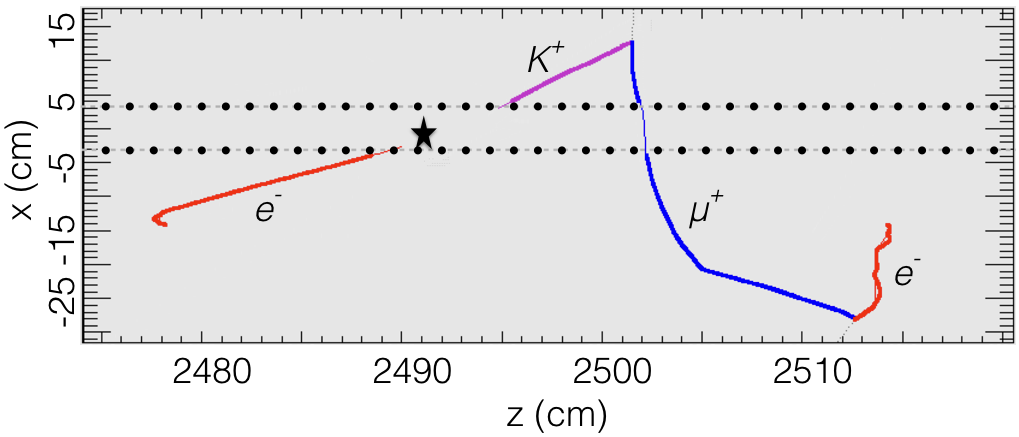
\includegraphics[width=0.8\textwidth]{KaonElecBigGap}
  \caption[A simulated $n \rightarrow K^{+} + e^{-}$ decay which occured in a gap between TPCs]
          {A simulated $n \rightarrow K^{+} + e^{-}$ decay which occured in a gap between TPCs. The path which the kaon produced in the decay took is shown as a purple line. The path which the muon produced by the decay of the kaon is shown as a blue line. The paths which the electrons in the event took are shown as red lines, the electron on the left is the electron produced in the neutron decay, whilst the one on the right is produced by the decay of the muon. The thin coloured lines, show track segments which were in uninstrumented parts of the detector, such as gaps between TPCs and APAs. The dotted black lines shows the gap between the TPCs, and the black star shows the location at which the decay occured. The distance between the first kaon energy deposition and the first electron energy deposition is found to be 10.7 cm. However, when the kaon and electrons tracks are extrapolated towards the true start position, the point of closest approach (PoCA) between the two tracks is found to be 0.67 cm, showing that they do infact have a common vertex, despite the seperation of the start points.} 
  \label{fig:NDK_Sig_KEBigGap}
\end{figure}

In the determination of whether a kaon track and an electron shower share a common vertex, the first requirement which is applied is whether the distance between the starts of the kaon track, and the electron shower, are seperated by less than 5 cm. A maximum seperation of 5 cm is used, as, if the two particles are produced in the centre of a TPC, a gap of 5 cm would require no energy depositions to be collected over approximately 10 collection wires. This is assumed to be unlikely during data taking, and cannot happen in the simulations considered here, as Monte Carlo truth information is used. As shown by Figure~\ref{fig:NDK_Sig_KEBigGap} however, it is possible for the kaon and electron to be seperated by more than 5 cm in signal events. To prevent events such as this being missed, a second criteria is applied to events with large seperations. Both the kaon and electron tracks, are extrapolated from their start and end points, and the minimum seperation of these extrapolated tracks is calculated. This is known as calculating the ``Point of Closest Approach'' (PoCA) between the two tracks, and if this PoCA is less than 2 cm, then the tracks are considered to have a common vertex which was missed. \\

When performing the fiducial cut, it is only applied to the outer edges of the cryostat, as if it were done with respect to the edge of every TPC in the far detector the loss of volume would be prohibitive. This means that the event shown in Figure~\ref{fig:NDK_CosmoBack_Raw} would not fail the fiducial cut, as the decay occured over 6 m away from the edge of the detector, but happened to be in a gap between two TPCs. The need for a fiducial cut is two fold, firstly the vast majority of cosmically induced events in the detector will have a charged particle, which was produced externally, entering the detector. Performing a fiducial cut will remove all of these events, and will then mean that the only cosmic background events which can induce a signal would involve either a significant amount of charge being missed, or a neutral particle entering the detector, and interacting far from the detector wall. Secondly, in order to calculate the kinetic energies of the particles produced in the nucleon decay, and also to perform particle identification, they must be fully contained within the detector. As such, if one of the particles produced in the nucleon decay escapes the detector then it's kinetic energy cannot be determined accurately, and if it is the kaon, or its decay products, then the particle cannot be identified using the method discussed in Section~\ref{sec:PID}. A fiducial cut of 2 cm is used, as the loss of volume is negligible in a detector which is scale of the DUNE FD, whilst also ensuring that a significant amount of charge would have to be missed for a particle which enters/escapes the detector to be incorrectly identified as being contained within the detector. \\

Once both the ancestry of energy depositions in the simulation, and the initial kinetic energies, have been correctly accounted for and calculated, it is possible to observe the distribution of background events, as the cuts outlined above are applied. The energy distribution of background events survivng the application of sequential cuts is shown in Figure~\ref{fig:NDK_CosmoBack_Raw}. The normalised energy distribution of background events surviving the application of sequential cuts is shown in Figure~\ref{fig:NDK_CosmoBack_Norm}. The distribution of normalised energies is found by dividing the number of events by the bin energy. \\

\begin{figure}[h!]
  \centering
  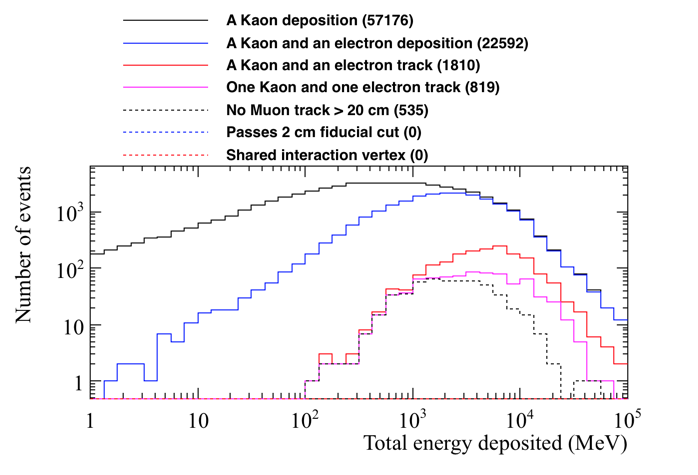
\includegraphics[width=0.8\textwidth]{CosmicBackground_EnergyDepCuts_Raw_2cmCut}
  \caption[The energy distribution of background events surviving the application of sequential cuts in the $n \rightarrow K^{+} + e^{-}$ channel]
          {The energy distribution of background events surviving the application of sequential cuts in the $n \rightarrow K^{+} + e^{-}$ channel. The total energy deposited in the detector is plotted on the $x$ axis.}
  \label{fig:NDK_CosmoBack_Raw}
\end{figure}

\begin{figure}[h!]
  \centering
  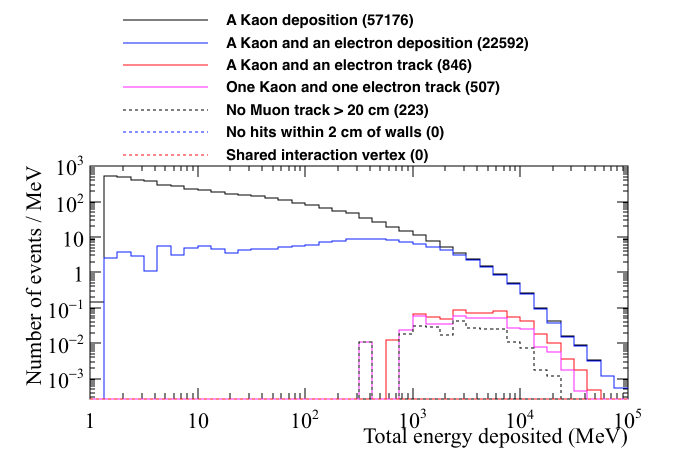
\includegraphics[width=0.8\textwidth]{CosmicBackground_EnergyDepCuts_Norm_2cmCut}
  \caption[The normalised energy distribution of background events surviving the application of sequential cuts in the $n \rightarrow K^{+} + e^{-}$ channel]
          {The normalised energy distribution of background events surviving the application of sequential cuts in the $n \rightarrow K^{+} + e^{-}$ channel. The total energy deposited in the detector is plotted on the $x$ axis. The normalised energy distribution has been found by dividing the number of events within a bin by the bin energy.}
  \label{fig:NDK_CosmoBack_Norm}
\end{figure}

From Figures~\ref{fig:NDK_CosmoBack_Raw} and~\ref{fig:NDK_CosmoBack_Norm}, it can be seen that there are no background events which could mimic a decay signature as there no events which survive the application of all cuts. This corresponds to a limit on the cosmogenic background to the $n \rightarrow K^{+} + e^{-}$ decay channel of XX$\times$10$^XX$. \\

It is interesting however, to observe the effect that relaxing the cuts after the presence of at least one kaon track and at least one electrons shower in the event has been confirmed. This allows for the effectiveness of each of the cuts to be observed. Initially, the four cuts which are applied afer kaon tracks, and electron showers, have been identified, are applied in isolation. The number of events surviving each of the cuts is shown in Table~\ref{tab:NDK_CosmoBack_EachCut}. \\

\begin{table}[h!]
  \caption[The number of events surviving isolated cuts which could mimic a $n \rightarrow K^{+} + e^{-}$ decay]
          {The number of events surviving isolated cuts which could mimic a $n \rightarrow K^{+} + e^{-}$ decay. Cuts are applied after it is found that the event contains at least one kaon track, and at least one electron shower present. This is found to be true for 845 events, representing the top line of the table. The fiducial cut of 2 cm is seen to remove all of the events considered.}
  \centering
  \label{tab:NDK_CosmoBack_EachCut}
  \begin{tabular}{c c}
    \toprule
        {Cut that is applied}                                & {Num. events survivng isolated cut} \\
        \midrule
        At least one kaon track, and electron shower         & 845                                 \\

        Only one kaon track, and only one electron shower    & 507                                 \\

        No muon track that is longer than 20 cm in length    & 339                                 \\

        No energy depositions within 2 cm of detector edge   & 0                                   \\

        The kaon and electron share a common vertex          & 85                                  \\
        \bottomrule
  \end{tabular}
\end{table}

The effectiveness of the fiducial cut is clearly apparent from Table~\ref{tab:NDK_CosmoBack_EachCut}, as it removes all 845 events where there is both a kaon track and an electron shower. It is for this reason that the loss in fiducial volume that it causes is accepted. The requirement made on the proximity of the kaon track and electron shower is also seen to be very effective at removing background events. It is found that of the 507 events that have a single kaon track, and a single electron shower, in only 41 of them would the kaon and electron be considered to have a common vertex. When the additional constraint of there not being a muon with a track length of more than 20 cm present in the event is applied, only 11 events would survive the cuts. This shows that the only way to remove all potential background events is to apply the fiducial cut, or to make the some of the other criteria stricter, such as reducing the seperation of the kaon track and the electron shower which constitutes a common vertex. \\

%********************************** % Fifth.Second Section  *************************************
\subsection{Signal events in the $n \rightarrow K^{+} + e^{-}$ decay channel} \label{sec:NDKSig}
It is important to confirm that the cuts developed do not adversely affect the identification of true nucleon decay events. For this reason a sample of 10,000 neutron decay events in the DUNE far detector were generated using GENIE. Neutron decays are generated at random positions within the detector volume, and so it is possible that the decay occurs in between TPC volumes, as shown in Figure~\ref{fig:NDK_Sig_KEBigGap}, or near the edge of the detector, as is shown in Figure~\ref{fig:NDK_Sig_KENearEdge}. \\

\begin{figure}[h!]
  \centering
  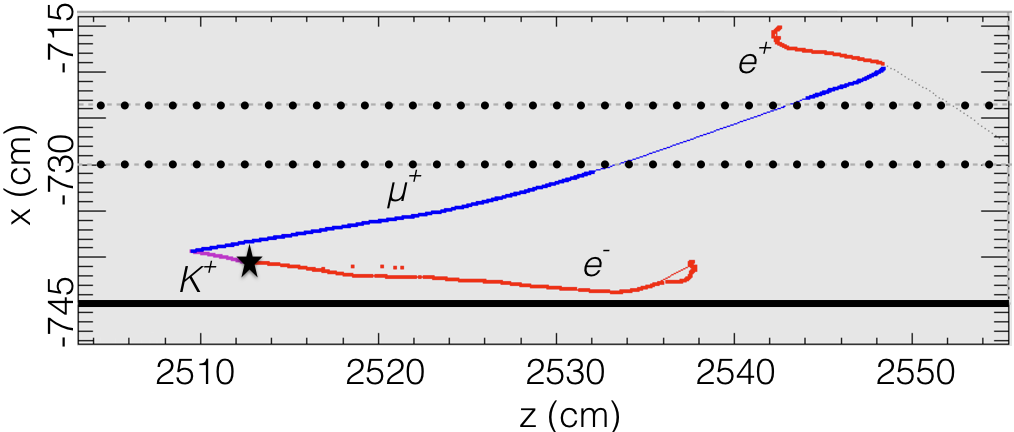
\includegraphics[width=0.8\textwidth]{KaonElecNearEdge}
  \caption[A simulated $n \rightarrow K^{+} + e^{-}$ decay which occured near the edge of the detector volume]
          {A simulated $n \rightarrow K^{+} + e^{-}$ decay which occured near the edge of the detector volume. The path which the kaon produced in the decay took is shown as a purple line. The path which the muon produced by the decay of the kaon is shown as a blue line. The paths which the electrons in the event took are shown as red lines, the electron on the left is the electron produced in the neutron decay, whilst the one on the right is produced by the decay of the muon. The thin coloured lines, show track segments which were in uninstrumented parts of the detector, such as gaps between TPCs and APAs. The dotted black lines shows the gap between the TPCs, and the solid black line shows the edge of the detector. The black star shows the location at which the decay occured. It can be seen that though the event is contained within the detector it is very close to the edge of the detector due to the location at which the decay occured.}
  \label{fig:NDK_Sig_KENearEdge}
\end{figure}

The analysis performed on the cosmogenic background was primarily designed to reject background events, whilst also attempting to not use cuts which would also affect signal efficiency. Therefore, it is hoped that the loss of signal events will be minimal. When running the analysis on the simulated signal events the same definitions for tracks, showers, and the ancestory of particles are used, as well as the same cuts that were outlined in Section~\ref{sec:NDKCosmBk}. \\

The energy distribution of the signal events survivng the application of the sequential cuts is shown in Figure~\ref{fig:NDK_Sig_Raw}, this is the equivalent of Figure~\ref{fig:NDK_CosmoBack_Raw} for the cosmogenic background sample. The normalised energy distribution of signal events surviving the application of sequential cuts is shown in Figure~\ref{fig:NDK_Sig_Norm}, this is the equivalent of Figure~\ref{fig:NDK_CosmoBack_Norm} for the cosmogenic background sample. As before, the distribution of normalised energies is found by dividing the number of events by the bin energy. \\

\begin{figure}[h!]
  \centering
  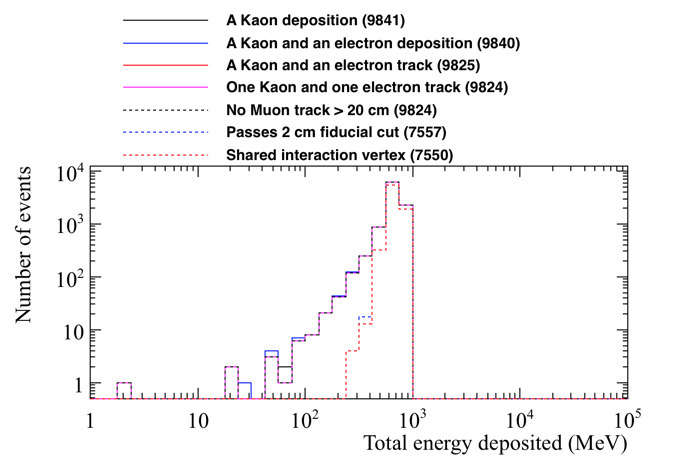
\includegraphics[width=0.8\textwidth]{NucleonDecay_EnergyDepCuts_Raw_2cmCut}
  \caption[The energy distribution of signal events surviving the application of sequential cuts in the $n \rightarrow K^{+} + e^{-}$ channel]
          {The energy distribution of signal events surviving the application of sequential cuts in the $n \rightarrow K^{+} + e^{-}$ channel. The total energy deposited in the detector is plotted on the $x$ axis.}
  \label{fig:NDK_Sig_Raw}
\end{figure}

\begin{figure}[h!]
  \centering
  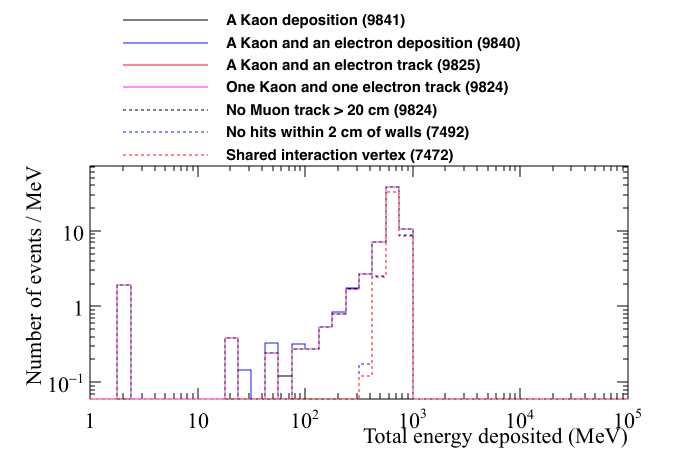
\includegraphics[width=0.8\textwidth]{NucleonDecay_EnergyDepCuts_Norm_2cmCut}
  \caption[The normalised energy distribution of signal events surviving the application of sequential cuts in the $n \rightarrow K^{+} + e^{-}$ channel]
          {The normalised energy distribution of signal events surviving the application of sequential cuts in the $n \rightarrow K^{+} + e^{-}$ channel. The total energy deposited in the detector is plotted on the $x$ axis. The normalised energy distribution has been found by dividing the number of events within a bin by the bin energy.}
  \label{fig:NDK_Sig_Norm}
\end{figure}

When comparing Figures~\ref{fig:NDK_Sig_Raw} and~\ref{fig:NDK_Sig_Norm} with Figures~\ref{fig:NDK_CosmoBack_Raw} and~\ref{fig:NDK_CosmoBack_Norm}, the most obvious difference is that when considering the nucleon decay events, the total energy deposited in the detector never exceeds 1 GeV, whilst in the cosmogenic background sample, the energy deposited in the detector frequently exceeds 1 GeV. This is something which one would expect, as the simulated neutrons decay at rest and so have a total energy of less than 1 GeV, meaning that there cannot be more than 1 GeV deposited in the detector. This is in stark contrast to the cosmogenic background, where the primary muons being generated have a mean energy of 283 GeV, as shown in Table~\ref{tab:MUSUNflux}. This means that many events will deposit sigificant amounts of energy in the detector, even if the primary muon narrowly misses the detector volume. \\

The initial cuts, requiring that both a kaon track and an electron shower are observed in the decay, show that there are occassions when either the kaon, or the electron, do not deposit energy in the detector. This affects very few events, though an example of one such event is shown in Figure~\ref{fig:NDK_Sig_MissedKaon}, where it can be seen that the kaon decayed before entering the active volume, and so no track was found for it. It would be very difficult to identify this event as a signal event, as the presence of the kaon could only be inferred from the muon originating from the gap between the APAs, and the energy deposited by the kaon will not be reconstructed. Further compounding the identification of this event as a signal event, is the fact that the electron produced in the nucleon decay scatters back into the gap between the APAs, and so a significant amount of its energy would not be reconstructed. \\

\begin{figure}[h!]
  \centering
  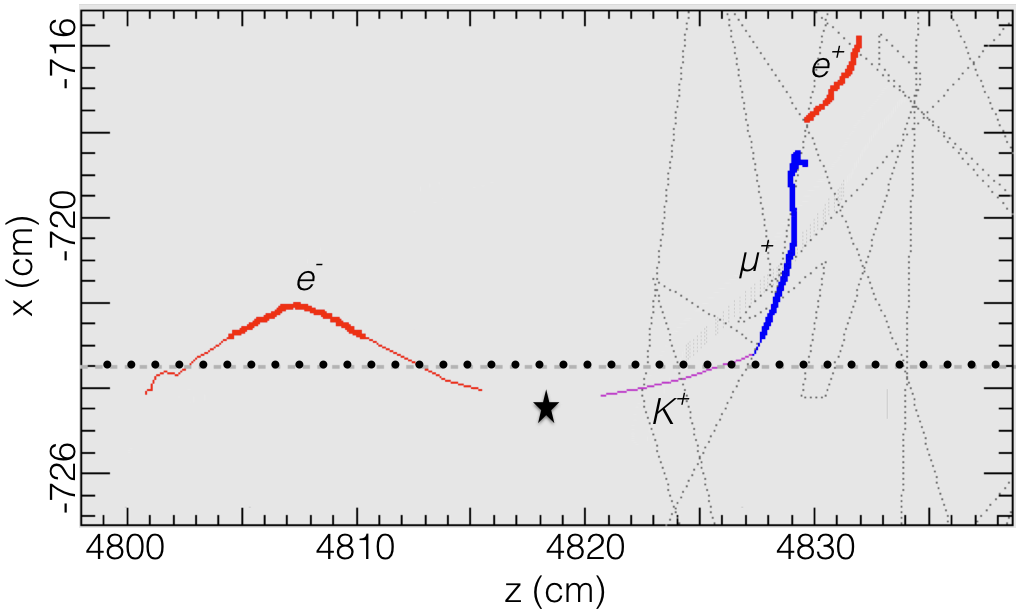
\includegraphics[width=0.8\textwidth]{MissedKaon}
  \caption[A simulated $n \rightarrow K^{+} + e^{-}$ decay where the kaon did not deposit any energy in the active volume]
          {A simulated $n \rightarrow K^{+} + e^{-}$ decay where the kaon did not deposit any energy in the active volume. The path which the kaon produced in the decay took is shown as a purple line. The path which the muon produced by the decay of the kaon is shown as a blue line. The paths which the electrons in the event took are shown as red lines, the electron on the left is the electron produced in the neutron decay, whilst the one on the right is produced by the decay of the muon. The thin coloured lines, show track segments which were in uninstrumented parts of the detector, such as gaps between TPCs and APAs. The dotted black lines shows the gap between the TPCs, and the solid black line shows the edge of the detector. The black star shows the location at which the decay occured. It can be seen that the kaon decayed before it entered the active volume of the detector, and so no track was found for it. A significant portion of the distance which the electron from the decay travelled was also outside the active volume of the detector.}
  \label{fig:NDK_Sig_MissedKaon}
\end{figure}

The number of events which are removed by the fiducial cut is concerning, as almost 20\% of events are removed due to it. This suggests that the cut is too strict. The reason for this, is that protons and neutrons are emitted from the nucleus in many of the simulated decays, and whilst the protons produced will create relatively short tracks, which are connected to the decay vertex, the neutrons will travel large distances, and cause energy depositions which are far away from the decay vertex. The faint dashed lines in Figure~\ref{fig:NDK_Sig_MissedKaon} show the spallation neutrons produced in the decay. It is preodiminantly the energy depositions from these spallation neutrons which are causing events to fail the ``no energy depositions within 2 cm of the detector edge'' cut. As a result it is likely that this cut needs to be relaxed, to instead be a a cut on the amount of energy deposited within 2 cm of the detector edge. Figure~\ref{fig:NDK_EDepNearEdge} shows the amount of energy deposited within 2 cm, 5 cm, and 10 cm of the detector edges, for the simulated nucelon decay events, and the cosmogenic background events. \\ 

\begin{figure}[h!]
  \centering
  \begin{subfigure}{0.75\textwidth}
    \centering
    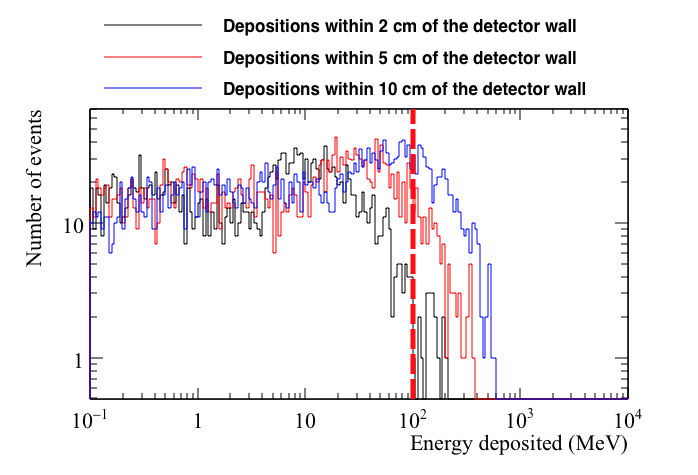
\includegraphics[width=\textwidth]{NucleonDecay_EDepNearEdges}
    \caption{The nucleon decay events.}
  \end{subfigure}
  % ========
  \begin{subfigure}{0.75\textwidth}
    \centering
    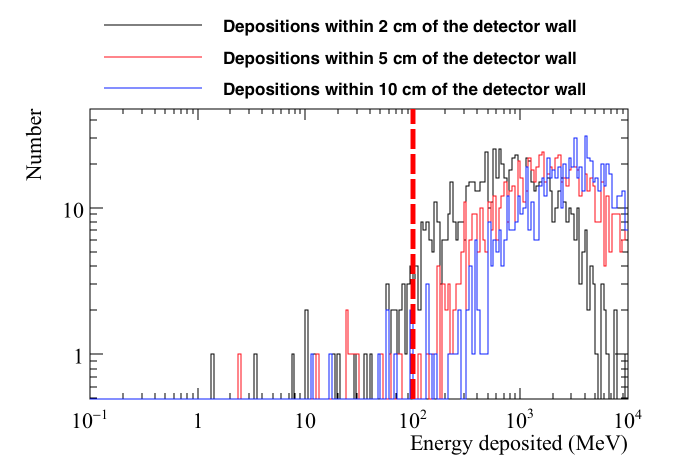
\includegraphics[width=\textwidth]{CosmicBackground_EDepNearEdges}
    \caption{The cosmogenic background events.}
  \end{subfigure}
  % ========
  \caption[The number of events, as a function of the energy deposited within 2 cm, 5 cm, and 10 cm of the detector edges.]
          {The number of events, as a function of the energy deposited within 2 cm, 5 cm, and 10 cm of the detector edges. Top shows the energies which were deposited for the simulated neutron decay events. Bottom shows the energies which were deposited in the simulated cosmogenic background events. The histograms are filled after the cut requiring that there is no muon with a track length of greater than 20 cm in the detector is applied. As such, the histograms are filled with 9824 and 223 events for the top and bottom histograms respectively. The dashed red line shows a preliminary cut on the energy deposited of 100 MeV.}
  \label{fig:NDK_EDepNearEdge}
\end{figure}

As can be seen from Figure~\ref{fig:NDK_EDepNearEdge}, the amount of energy deposited near the detector edges is very different in the nucleon decay and cosmogenic background events. As such, they can be cleanly seperated, and so a very conservative cut, requiring no more than 100 MeV of energy to be deposited within 2 cm of the detector edge, can be used. There are very entries in the figure for the simulated neutron decay events, because, as shown in Figures~\ref{NucleonDecay_EnergyDepCuts_Raw_2cmCut} and~\ref{NucleonDecay_EnergyDepCuts_Norm_2cmCut}, there are 7492 events for which there are no depositions within 2 cm of the detector edge. Requiring that there be no more 100 MeV of energy deposited within 2 cm of the detector edges, removes only 19 of the 9824 signal events, whilst only 18 out of the 223 cosmic background events meet this requirement. Whilst this does mean that the fiducial cut is no longer as effective at removing the cosmic background sample, it does not cause the huge loss of signal events which was seen when the hard cut, of no energy depositions within 2 cm of the detector edge, was used. It is also important to remember that the requirement that the kaon and electron share a common vertex, as well as cuts on the energy deposition profiles, will still be applied to these 18 background events. It will be seen in Section~\ref{sec:NDKEnCosmBk}, that no events survive the appliction of these cuts. \\

The definition used to decide if the start of the kaon track, and the start of the electron shower, share a common vertex seems to be a reasonable requirement, as almost all of the signal events satisfy this definition. The distance between the start of the kaon track, and the start of the electron shower is shown in Figure~\ref{fig:NDK_Sig_KEDist}. It can be seen that the seperation between the two particles is very small (<0.1 cm) in most events. However, there are some events where the seperations are very large (>10 cm). As discussed earlier, the decays in these events occur in the gaps between TPCs, such as that shown in Figure~\ref{fig:NDK_Sig_KEBigGap}. When the requirement that the kaon and electron track have a PoCA of less than 2 cm is then applied to these events, most of them are then shown to have a common interaction vertex. This is found to be the case for the event shown in Figure~\ref{fig:NDK_Sig_KEBigGap}. However, in some events the kaon track, and the electron shower, are still found to not have a common interaction vertex. Handscanning of these events shows that particles undergo scattering before entering the active volume, and so by the time the energy depositions are collected, their trajectories are no longer closely alligned, causing them to have large values for the PoCA which is calculated. \\

\begin{figure}[h!]
  \centering
  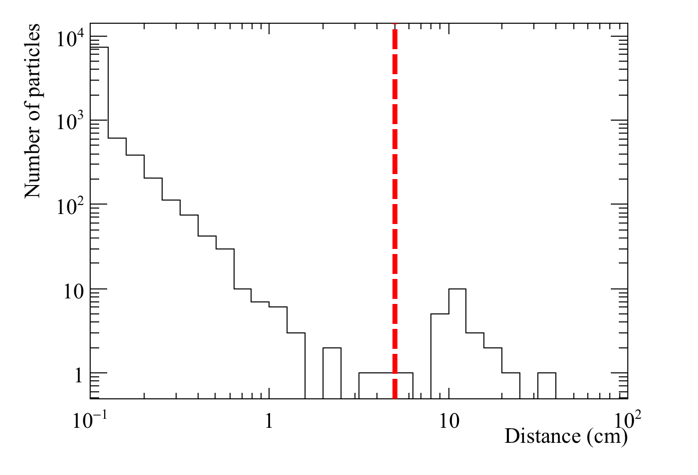
\includegraphics[width=0.8\textwidth]{NucleonDecay_KaonElecSep}
  \caption[The seperation of the kaon and the electron produced in the $n \rightarrow K^{+} + e^{-}$ decay channel]
          {The seperation of the kaon and the electron produced in the $n \rightarrow K^{+} + e^{-}$ decay channel. The dashed red line, drawn at a seperation of 5 cm, shows the maximum possible seperation a kaon and an electron could have, and still be considered to have a common vertex.}
  \label{fig:NDK_Sig_KEDist}
\end{figure}

The normalised energy distributions of simulated decay events, and simulated cosmogenic background events, after the fiducial cut is changed to be a limit of 100 MeV of energy deposited within 2 cm of the detector edge, is shown in Figure~\ref{fig:NDK_FidCut_EnLim}. As before, the distribution of normalised energies is found by dividing the number of events by the bin energy. \\

\begin{figure}[h!]
  \centering
  \begin{subfigure}{0.8\textwidth}
    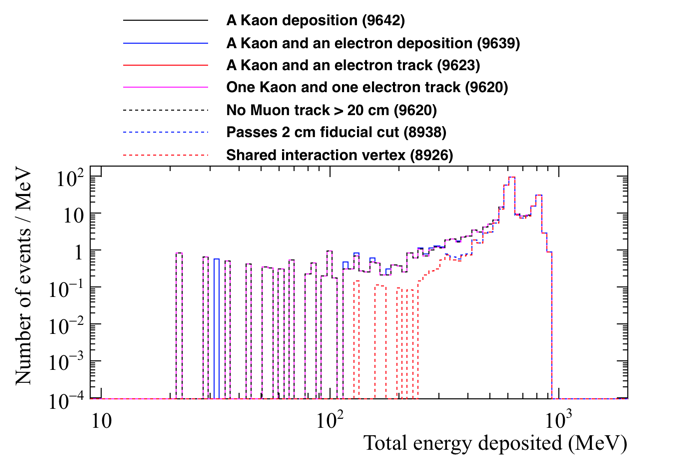
\includegraphics[width=\textwidth]{NucleonDecay_EnergyDepCuts_Norm}
    \caption{The normalised energy distribution of signal events.}
    \label{fig:NDK_FidCut_EnLim_Sig}
  \end{subfigure}
  % ========
  \begin{subfigure}{0.8\textwidth}
    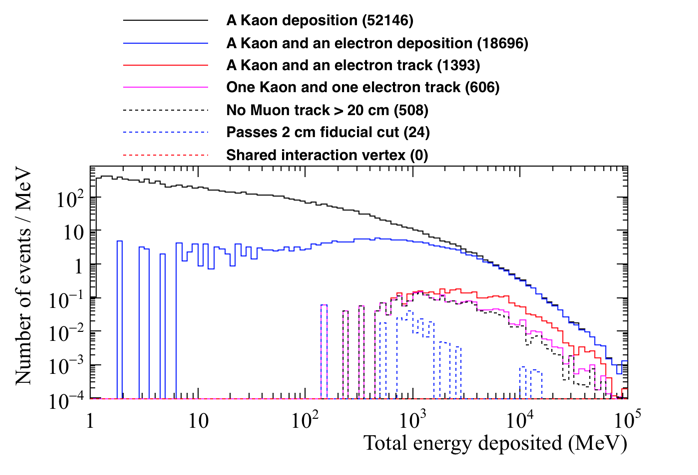
\includegraphics[width=\textwidth]{CosmicBackground_EnergyDepCuts_Norm}
    \caption{The normalised energy distribution of cosmic background events.}
    \label{fig:NDK_FidCut_EnLim_Cosmo}
  \end{subfigure}
  \caption[The normalised energy distribution of signal events, and cosmic background events, surviving the application of sequential cuts, after the fiducial cut is modified]
          {The normalised energy distribution of signal events, and cosmic background events, surviving the application of sequential cuts, after the fiducial cut is modified. The total energy deposited in the detector is plotted on the $x$ axis. The normalised energy distribution has been found by dividing the number of events within a bin by the bin energy.}
  \label{fig:NDK_FidCut_EnLim}
\end{figure}

The number of signal events which are removed by the cuts can be seen to be much more reasonable after the fiducial cut is modified, as less than 2.5\% of signal events are removed as cuts are applied. It is seen that in many of the simualted decay events which fail the cuts, at least one of the kaon, or the electron, are not contained in the detector. This means that, either no depositions are found for the particle, or it deposits significant amounts of energy as it leaves the detector. \\

It can be seen that though 4 of the cosmic background events pass the application of all cuts, the total energy deposited in the detector is not less than 1 GeV in any of these events. This means that the total energy deposited in the detector is more than the rest mass of a neutron, and so the event is not consistent with being from the decay of a neutron at rest. However, it is still prudent to determine the expected energy deposition distribution for the signal events, to ensure that a clean seperation can be observed between the signal and background events.  \\

%********************************** % Fifth.Second Section  *************************************
\subsection{Energy constraints on the cosmogenic background to the $n \rightarrow K^{+} + e^{-}$ decay channel} \label{sec:NDKEnCosmBk}
As outlined in Section~\ref{sec:NDKCosmBk}, it is possible to exclude background events from signal events, using the distribution of how energy is deposited in the detector. The energy criteria which were previously outlined were;
\begin{itemize}
\item The energy directly deposited by the kaon.
\item The energy deposited by the kaon decay products.
\item The energy directly deposited by the electron.
\item The energy deposited near the shared kaon and electron vertex
\item The energy deposited in the detector which does not fit any of the above criteria.
\end{itemize}
Following the earlier discussions in Section~\ref{sec:DUNENDK}, it should be clear that the energy directly deposited by the kaon corresponds to the sum of all energy depositions which are due to the kaon or its interaction products. Equivalently, the energy directly deposited by the electron corresponds to the sum of all energy depositions which are due to the electron as it showers, and any particles created as a result of the shower. The energy deposited by the kaon decay products, would include all depositions by the muon and subsequent electron, in the case that the kaon decayed via $k^{+} \rightarrow \mu^{+} + \nu_{\mu}$, and then the muon decayed via $\mu^{+} \rightarrow e^{+} + \nu_{e} + \nu_{\mu}$. The energy deposited near the shared kaon and electron vertex, would primarily consist of energy depositions due to spallation products. The depositions due to spallations products would largely be due to protons, though may also include some depositions due to the neutrons too, if they deposit energy near the vertex. Any depositions within 5 cm of the kaon and electron vertex are considered as 'near.' The final criteria, of any depositions which do not fit the above description, would largely consist of energy depositions due to the spallation neutrons in the decay sample. However, in the cosmic background sample, this would include all depositions by muons, pions, and any other particles which enter the detector. \\

In presenting the seperation of simulated cosmic background events and simulated neutron decay events, the important distributions to consider are as follows:
\begin{itemize}
\item The energy directly deposited by the kaon, against the energy directly deposited by the electron. This is shown in Figure~\ref{fig:NDK_Kaon_Elec_EDist}.
\item The energy directly deposited by the kaon, plus the energy directly deposited by the electron, against the energy deposited near the shared kaon and electron vertex. This is in Figure.
\item The energy deposited by the kaon, including decay products, against the energy deposited in the detector which does not fit any of the other criteria. This is shown in Figure.
\item The energy deposited by the kaon, including decay products, plus the energy directly deposited by the electron, plus the energy deposited near the shared kaon and electron vertex, against the energy deposited in the detector which does not fit any of the other criteria. This is shown in Figure.
\end{itemize}
Each will be discussed in turn below. When looking at the figures presented, the events which pass all cuts in the simulated decay sample have been plotted with much smaller markers, so as to not to allow the events which fail the cuts to be visible. The markers have also been plotted so as to have the earlier cuts in the foreground in the nucleon decay sample, and the later cuts to be in the foreground in the cosmic background sample. This was done so as to prevent the events which fail (pass) the cuts, from being overwhelmed by the more numberous events which pass (fail) the cuts, in the simulated nucleon decay (cosmic background) sample. \\

% ========== Kaon vs Elec
\begin{figure}[h!]
  \centering
  \begin{subfigure}{0.8\textwidth}
    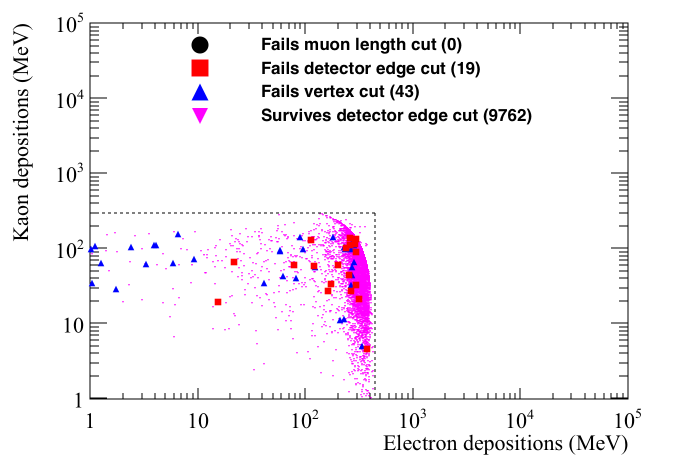
\includegraphics[width=\textwidth]{NucleonDecay_Kaon_vs_Elec_Can}
    \caption{The energy distribution of signal events.}
    \label{fig:NDK_Kaon_Elec_EDist_Sig}
  \end{subfigure}
  % ========
  \begin{subfigure}{0.8\textwidth}
    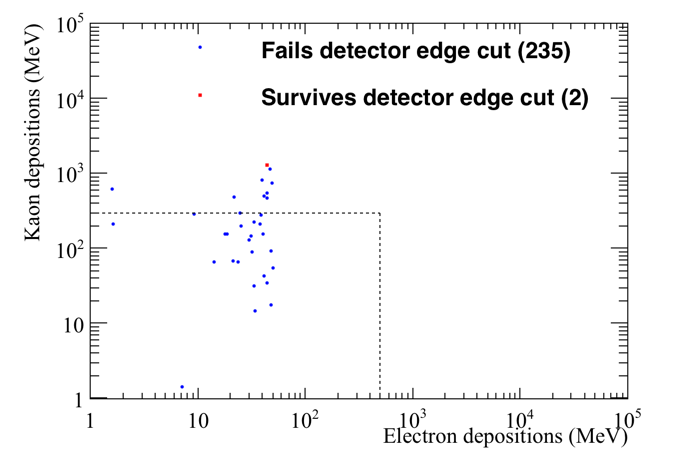
\includegraphics[width=\textwidth]{CosmicBackground_Kaon_vs_Elec_Can}
    \caption{The energy distribution of cosmic background events.}
    \label{fig:NDK_Kaon_Elec_EDist_Cosmo}
  \end{subfigure}
  \caption[The energy directly deposited by kaons, as a function of the energy directly deposited by electrons, in the simulated nucleon decay, and cosmic background samples]
          {The energy directly deposited by kaons, as a function of the energy directly deposited by electrons, in the simulated nucleon decay, and cosmic background samples. The events failing the application of the muon length (black circle), fiducial (red box) and vertex (blue triangle) cuts, as well as the events passing all cuts (pink triangle) are shown.}
  \label{fig:NDK_Kaon_Elec_EDist}
\end{figure}

% ========== Kaon + Elec vs Near
\begin{figure}[h!]
  \centering
  \begin{subfigure}{0.8\textwidth}
    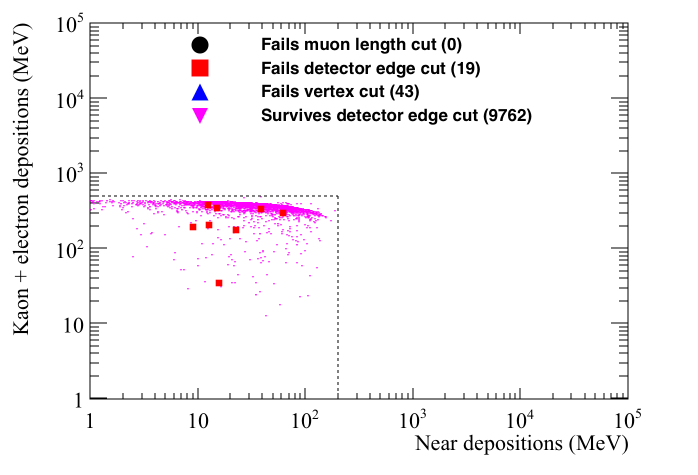
\includegraphics[width=\textwidth]{NucleonDecay_KaonElec_vs_Near_Can}
    \caption{The energy distribution of signal events.}
    \label{fig:NDK_KaonElec_Near_EDist_Sig}
  \end{subfigure}
  % ========
  \begin{subfigure}{0.8\textwidth}
    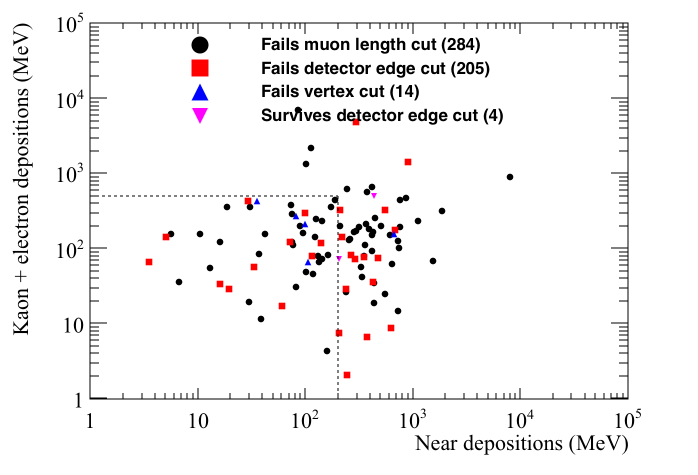
\includegraphics[width=\textwidth]{CosmicBackground_KaonElec_vs_Near_Can}
    \caption{The energy distribution of cosmic background events.}
    \label{fig:NDK_KaonElec_Near_EDist_Cosmo}
  \end{subfigure}
  \caption[The energy directly deposited by kaons, plus the energy directly deposited by electrons, as a function of the energy deposited near the kaon and electron vertex, in the simulated nucleon decay, and cosmic background samples]
          {The energy directly deposited by kaons, plus the energy directly deposited by electrons, as a function of the energy deposited near the kaon and electron vertex, in the simulated nucleon decay, and cosmic background samples. The events failing the application of the muon length (black circle), fiducial (red box) and vertex (blue triangle) cuts, as well as the events passing all cuts (pink triangle) are shown.}
  \label{fig:NDK_KaonElec_Near_EDist}
\end{figure}

% ========== Kaon + Kaon Decay vs Other
\begin{figure}[h!]
  \centering
  \begin{subfigure}{0.8\textwidth}
    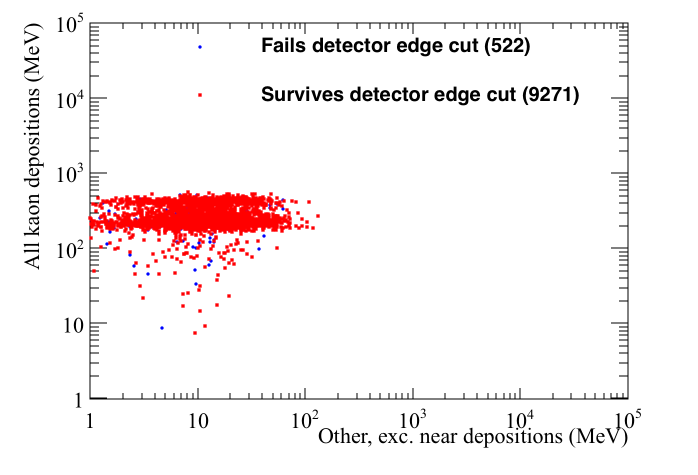
\includegraphics[width=\textwidth]{NucleonDecay_AllKaon_vs_Other_Can}
    \caption{The energy distribution of signal events.}
    \label{fig:NDK_AllKaon_Other_EDist_Sig}
  \end{subfigure}
  % ========
  \begin{subfigure}{0.8\textwidth}
    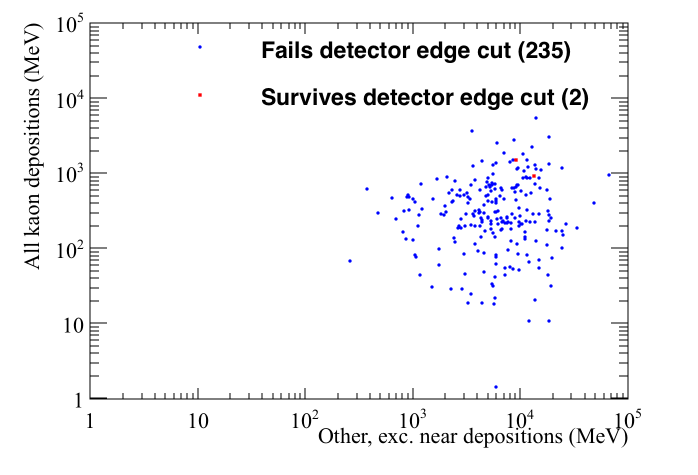
\includegraphics[width=\textwidth]{CosmicBackground_AllKaon_vs_Other_Can}
    \caption{The energy distribution of cosmic background events.}
    \label{fig:NDK_AllKaon_Other_EDist_Cosmo}
  \end{subfigure}
  \caption[The energy directly deposited by kaons, plus the energy deposited by the kaon decay products, as a function of the energy depositions which do not fit any of the other criteria, in the simulated nucleon decay, and cosmic background samples]
          {The energy directly deposited by kaons, plus the energy deposited by the kaon decay products, as a function of the energy depositions which do not fit any of the other criteria, in the simulated nucleon decay, and cosmic background samples. The events failing the application of the muon length (black circle), fiducial (red box) and vertex (blue triangle) cuts, as well as the events passing all cuts (pink triangle) are shown.}
  \label{fig:NDK_AllKaon_Other_EDist}
\end{figure}

% ========== Kaon + Kaon Decay + Elec + Near vs Other
\begin{figure}[h!]
  \centering
  \begin{subfigure}{0.8\textwidth}
    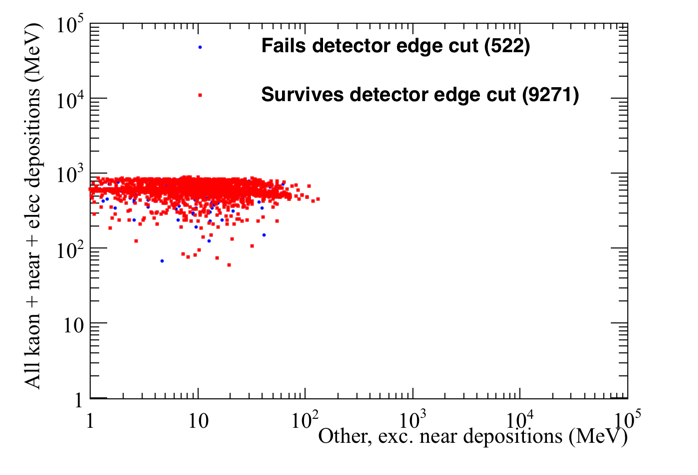
\includegraphics[width=\textwidth]{NucleonDecay_AllKaonNearElec_vs_Other_Can}
    \caption{The energy distribution of signal events.}
    \label{fig:NDK_AllEDep_Other_EDist_Sig}
  \end{subfigure}
  % ========
  \begin{subfigure}{0.8\textwidth}
    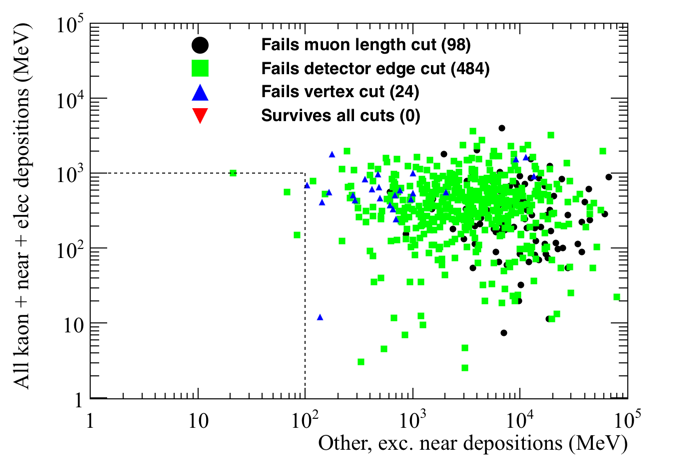
\includegraphics[width=\textwidth]{CosmicBackground_AllKaonNearElec_vs_Other_Can}
    \caption{The energy distribution of cosmic background events.}
    \label{fig:NDK_Kaon_AllEDep_Other_Cosmo}
  \end{subfigure}
  \caption[The energy directly deposited by kaons, plus the energy deposited by the kaon decay products, plus the energy directly deposited by electrons, plus the energy deposited near the kaon and electron vertex, as a function of the energy depositions which do not fit any of the other criteria, in the simulated nucleon decay, and cosmic background samples]
          {The energy directly deposited by kaons, plus the energy deposited by the kaon decay products, plus the energy directly deposited by electrons, plus the energy deposited near the kaon and electron vertex, as a function of the energy depositions which do not fit any of the other criteria, in the simulated nucleon decay, and cosmic background samples. The events failing the application of the muon length (black circle), fiducial (red box) and vertex (blue triangle) cuts, as well as the events passing all cuts (pink triangle) are shown.}
  \label{fig:NDK_AllEDep_Other_EDist}
\end{figure}

% ========== Kaon vs Elec
From Figure~\ref{fig:NDK_Kaon_Elec_EDist} it can be seen that the electron energy distribution in the cosmic background sample is very different from the one seen in the simulated neutron decay sample. This is shown by energies deposited by electrons in the decay sample being tightly concentrated between 200 and 400 MeV, whilst in the cosmic background sample, the energy deposited by the electron is always less than 50 MeV. Many of the electrons in the cosmic background sample deposit less than 1 MeV of energy in the detector, and so are not shown here. This is why the events where the kaon and electron share a common vertex are not shown in the cosmic background sample. Realistically, these electrons are unlikely to be reconstructed due to their extremely low energies. From Figure~\ref{fig:NDK_Kaon_Elec_EDist_Sig}, it can be seen that some of the electrons produced in the nucleon decay events also deposit very little energy in the detector, though these events generally fail either the fiducial cut, or the vertex cut. An explanation as to why these events fail the cuts was presented in Section~\ref{sec:NDKSig}. \\

% ========== Kaon + Elec vs Near
From Figure~\ref{fig:NDK_KaonElec_Near_EDist} it can be seen that for the simulated nucleon decay events, as the energy deposited near the kaon and electron vertex increases, the sum of the energy deposited by the kaon and electron decreases. This is reasonable, because, when the spallation protons and neutrons have more energy, the kaon and electron will have less energy, due to conservation of energy. The decrease in the energy deposited by the kaon and the electron, is roughly consistent with the increase in energy deposited near their shared vertex. This means that the sum of the three energies is generally around 450 MeV. \\

% ========== Kaon + Kaon Decay vs Other
Figure~\ref{fig:NDK_AllKaon_Other_EDist} shows. \\

% ========== Kaon + Kaon Decay + Elec + Near vs Other
Figure~\ref{fig:NDK_AllEDep_Other_EDist} shows. \\

%********************************** % Fifth.Third Section  *************************************
\subsection{Future improvements to nucleon decay studies} \label{sec:NDKImprov}
Thus far the nucleon decay studies have been performed on the Monte Carlo truth information, and so have not used reconstructed objects such as tracks. The extension of the analyses to include work on tracks is an important next step as then the full analysis which would be applied on real data can be tested. Preliminary studies have begun on hit reconstruction, and involve running a filter on the muons used in the earlier analyses. This is because the number of events which are saved to disk would be prohibitive to running the full reconstruction process. As such, only events which meet the following criteria will be reconstructed~\citep{CosmoJanCollabMeeting};
\begin{itemize}
\item A minimum of 10 MeV deposited in the detector volume.
\item A maximum of 3,000 MeV deposited in the detector volume.
\item A maximum of 5 MeV deposited within 10 cm of the detector edge.
\end{itemize}
These criteria are designed to be broad enough that the full range of nucleon decay modes can be studied, including di-nucleon decay modes, hence the maximum deposited energy greatly exceeding the rest mass of a single nucleon. \\
